\chapter{Background Knowledge}
\label{BackgroundKnowledgeCh}

This chapter will introduce the necessary background knowledge to follow the
theoretical derivations later.

\section{Probability Theory and Statistics}

We go over the rules of probability and statistics.

\subsection{Rules and Theorems}

Rules of probability that will be useful to us are the following, if we let $X
\in \mathcal{X}$ be a random variable and $p(X)$ the probability distribution with
respect to this variable, then
\begin{description}
\item[Unit volume]
  \begin{equation}
    \label{eq:unit_vol_prob_axiom}
    \int_{\mathcal{X}}p(X) \dif X = 1
  \end{equation}
\item[Non-negativity]
  \begin{equation}
    \label{eq:non_neg_of_prob}
    p(X) \geq 0
  \end{equation}
\end{description}
where the integral is interpreted as the Lebesgue integral if $X$ is continuous and as
a sum over the possible values of $X$ if it is discrete.

Most manipulations of random variables reduces to the following two rules of
probability: given two random variables $X, Y$ defined on the domains $\mathcal{X}, \mathcal{Y}$ respectively, then
\begin{description}
\item[Sum rule]
  \begin{equation}
    \label{eq:sum_rule}
    p(X) = \int_{\mathcal{Y}}p(X, Y) \dif Y
  \end{equation}
\item[Product rule]
  \begin{equation}
    \label{eq:product_rule}
    p(X, Y) = p(Y | X)p(X)
  \end{equation}
\end{description}.
The product rule leads directly to Bayes Rule
\begin{description}
\item[Bayes Rule]
  \begin{equation}
    \label{eq:bayes_rule}
    p(X | Y) = \frac{p(Y | X)p(X)}{p(Y)}
  \end{equation}
\end{description}.

Two very important operations involving probabilities of random variables are
those of \textit{Expectation} and \textit{Covariance}. Assume $X \in \mathcal{X}$ is
a random variable with probability distribution $p(X)$ and $f : \mathcal{X} \to
\mathbb{R}$:
\begin{description}
\item[Expectation]
  \begin{equation}
    \label{eq:expectation}
    \E_X[f] = \int_{\mathcal{X}} f(X) p(X) \dif X
  \end{equation}
\item[Covariance]
  \begin{equation}
    \label{eq:covariance}
    \Cov(X, Y) = \E_{XY}[(X - \E_X[X])(Y - \E_Y[Y])]
  \end{equation}
\end{description}
We then define the variance operator as:
\begin{description}
\item[Variance]
  \begin{equation}
    \label{eq:variance}
    \Var(X) = \Cov(X, X)
  \end{equation}
\end{description}
The generalisation from $f: \mathcal{X} \to \mathbb{R}$ to $f: \mathcal{X} \to
\mathbb{R}^n$ is defined in the straightforward manner. If $\bm{f} =
f(X)$ then:
\begin{equation*}
  \E_X
  \begin{bmatrix}
    \bm{f}_1 \\
    \vdots \\
    \bm{f}_n \\
  \end{bmatrix} =
  \begin{bmatrix}
    \E_X \bm{f}_1 \\
    \vdots \\
    \E_X \bm{f}_n \\
  \end{bmatrix}
\end{equation*}
similarly $\Cov(\bm{f})$ is a $D \times D$-dimensional matrix where
$\Cov(\bm{f})_{i,j} = \Cov(\bm{f}_i, \bm{f}_j)$\cite{Bishop:2006}.

\subsection{The Gaussian Distribution}

For a $D$-dimensional random vector $\bm{X}$, the multivariate Gaussian
distribution takes the form
\begin{equation}
  \label{eq:Gaussian_dist}
  \mathcal{N}(\bm{X} | \bm{\mu}, \bm{\Sigma}) = \frac{1}{(2\pi)^{D/2}}\frac{1}{|\bm{\Sigma}|^{1/2}}\exp\left( -\frac{1}{2}(\bm{X} - \bm{\mu})^T\bm{\Sigma}^{-1}(\bm{X} - \bm{\mu})\right)
\end{equation}
where $\bm{\mu}$ is a $D$-dimensional mean vector, $\bm{\Sigma}$ is a $D \times
D$ dimensional positive definite covariance matrix, and $|\bm{\Sigma}|$ denotes
the determinant of $\bm{\Sigma}$. It is straightforward to show that these
parameters correspond to the mean and covariance as defined in equations
\eqref{eq:expectation} and \eqref{eq:covariance}\cite{}.

The Gaussian distribution can be seen as a unit $D$-dimensional cube which is
translated, sheared and rotated, giving rise to the fact that we can write any
Gaussianly distributed random variable $\bm{x} \sim \mathcal{N}(\bm{x} |
\bm{\mu}, \bm{\Sigma})$ as a linear combination of a unit Gaussian random
variable $\bm{z} \sim \mathcal{N}(\bm{x} | \bm{0}_D, \bm{I}_{D \times D})$. If
we let $\bm{\Lambda} \bm{\Lambda}^{\top} = \bm{\Sigma}$ be the Cholesky
decomposition\cite[p.~100-102]{Press:2007:NRE:1403886} of $\bm{\Sigma}$, then we
also have that
\begin{equation}
  \label{eq:sample_x}
  \bm{x} = \bm{\mu} + \bm{\Lambda}\bm{z}
\end{equation},
where the equality is in terms of distribution. If we further assume that
$\bm{x}$ is parametrised by $\bm{\mu}$ and $\bm{\Sigma}$ such that $\bm{\Sigma}$
is diagonal positive definite with diagonal $\bm{\sigma}$, then $\bm{\Sigma} =
\bm{\sigma} \odot \bm{I}_{D \times D}$. Finally this means that if we want to
sample a random variable $\bm{x}$ with diagonal covariance structure, then we
can do this by sampling a unit normal $\bm{z}$ which we then transform, which we can express as
\begin{equation}
  \label{eq:sample_x_diag_covariance}
  \bm{x} = \bm{\mu} + \bm{\sigma} \odot \bm{z} \sim \mathcal{N}(\bm{\mu}, \bm{\sigma} \odot \bm{I}_{D \times D})
\end{equation}

As the Gaussian distribution is part of the exponential family, the density of
joint distribution of iid Gaussian variables are themselves Gaussian distributed
where the natural parameters of this joint distribution is the sum of the
natural parameters of each random variable in the joint. In particular for the
Gaussian distribution, this means that if we have a collection of iid gaussian
random variables $\{\bm{x}_i\}_i^n$, such that $\bm{x}_i \sim
\mathcal{N}(\bm{x}_i | \bm{\mu}_i, \bm{\Sigma}_{i})$, then the joint
can be found to be Gaussian distributed as
\begin{equation*}
  \mathcal{N}(\bm{\mu}, \bm{\Sigma})
\end{equation*},
where
\begin{align}
  \bm{\Sigma} & = \left( \sum_i^n \bm{\Sigma}_i^{-1} \right)^{-1} \label{eq:joint_indep_normal_covariance}\\ 
  \bm{\mu} & = \bm{\Sigma}\left( \sum_i^n \bm{\Sigma}^{-1} \bm{\mu}_i \right) \label{eq:joint_indep_normal_mean}
\end{align}\cite[p.~78-84]{Bishop:2006}.

In the case of two random variables distributed according to the form as laid
out in \eqref{eq:sample_x}, $\bm{x} \sim
\mathcal{N}(\mathcal{N}(\bm{\mu}_{\bm{x}}, \bm{\sigma}_{\bm{x}} \odot \bm{I}))$
and $\bm{y} \sim \mathcal{N}(\mathcal{N}(\bm{\mu}_{\bm{y}}, \bm{\sigma}_{\bm{y}}
\odot \bm{I}))$ we have that the resulting distribution $p(\bm{x}, \bm{y}) =
p(\bm{x})p(\bm{y})$ is distributed such that
\begin{equation*}
  p(\bm{x}, \bm{y}) = \mathcal{N}(\bm{\mu}_{\bm{x}, \bm{y}}, \bm{\sigma}_{\bm{x}, \bm{y}})
\end{equation*}
where
\begin{align}
  \bm{\sigma}_{\bm{x}, \bm{y}} & = \frac{1}{\bm{\sigma}_{\bm{x}}^{-1} + \bm{\sigma}_{\bm{y}}^{-1}} \label{eq:joint_indep_normal_covariance_diag}\\
  \bm{\mu}_{\bm{x}, \bm{y}} & = \frac{\bm{\sigma}_{\bm{x}}^{-1}\bm{\mu}_{\bm{x}} + \bm{\sigma}_{\bm{y}}^{-1}\bm{\mu}_{\bm{y}}}{\bm{\sigma}_{\bm{x}}^{-1} + \bm{\sigma}_{\bm{y}}^{-1}} \label{eq:joint_indep_normal_mean_diag}
\end{align}.

\subsection{Maximum Likelihood Estimation}

Assume we have a model $\mathcal{M}$ parametrised by $\bm{\theta}$ constrained
to live in the parameter space $\bm{\Theta}$. Given data $\mathcal{D}$ we want
to be able to fit the parameters $\bm{\theta}$ such that these generalise to
unseen data. The MLE of of the parameters of the model is defined to be
\begin{equation}
  \label{eq:MLE}
  \hat{\bm{\theta}}_{ML} = \argmax_{\bm{\theta} \in \bm{\Theta}}\mathcal{L}(\bm{\theta}; \mathcal{D})
\end{equation}
.

While the original MLE is defined in terms of the likelihood function
$\mathcal{L}(\bm{\theta}; \mathcal{D})$, it's often more practical to work with
the logarithm of this function, the log-likelihood function $\ell(\bm{\theta} ;
\mathcal{D})$. Using the common assumption of i.i.d datapoints, the joint
distribution becomes a product of individual probabilities for each datapoint,
\begin{equation}
  \label{eq:likelihood}
  \mathcal{L}(\bm{\theta} | \mathcal{D}) = p(\bm{x}_1, \dots, \bm{x}_n | \bm{\theta}) = \prod_i^n p(\bm{x}_i | \bm{\theta})
\end{equation}.
Using the log-likelihood we transform this product into a form involving sums
\begin{equation}
  \label{eq:log-likelihood}
  \ell(\bm{\theta} | \mathcal{D}) = \log \mathcal{L}(\bm{\theta} | \mathcal{D}) = \sum_i^n \log p(\bm{x}_i)
\end{equation}.
Besides from simplifying notation and calculation, it has the added benefit of
reducing the risk of arithmetic underflow due to the small magnitude of
individual probabilities\footnote{Also, with the use of the log-sum-exp-trick,
  \begin{equation*}
    \log \sum_{i=1}^n \exp(x_n) = \max_i x_i + \log \sum_{i=1}^n \exp(x_n - \max_i x_i)
  \end{equation*}
  this problem can be reduced even further}.

MLE estimators have a number of nice properties such as consistency and
asymptotic normality, however, the optimization problem itself is often
non-convex, making it hard to find the actual estimator\cite{CaseBerg:01}.

\subsection{Graphical models}
tool for probabilistic modelling is the notion of using
diagrams to specify the conditional relationships between random variables. A
graphical model is a diagrammatic way of specifying this relationship by
creating a Directed Acyclic Graph, a directed graph without any cycles. This
representation is called a \textit{Graphical Model} and provide a powerful way
to visualize the structure of the probabilistic model and also how to use and
abuse the structure of the model in order to infer variables in a computationally efficient way.

A graph in this setting consists of a set of \textit{vertices} connected by
\textit{edges}, following the notation and nomenclature of graph theory as used
in mathematics. While there are many different kinds of graphical models
depending on the type of graph structure used (directed graphical models,
undirected graphical models, factor graphs, etc.), we will only focus on the
subset of graphical models called directed graphical models.

Directed graphical models specify how the joint distribution of a set of random
variables $\mathcal{X}$ factors in a conditional manner. In general, the
relationship between a given directed graph and the corresponding distribution
over the variables in $\mathcal{X}$ is such that the join distribution defined
by the graph is given by the product, over all vertices of the graph, of a
conditional distribution for each vertex conditioned on the variables
corresponding to the parents of that vertex in the graph. So for a graph with
$K$ vertices, the joint distribution is give by
\begin{equation}
  \label{eq:dir_graph_model_dist}
  p(\mathcal{X}) = \prod_{k=1}^K p(x_k | \text{pa}(x_k))
\end{equation}
where $\text{pa}(x_k)$ is defined as the set of random variables corresponding
to the parent vertices of the random variable $x_k$.

Although a graphical model is completely defined in terms of it's vertex and
edge set, it is really the most powerful when visualized as a diagram. As an
example I will repeat the above formulation in the context of the directed
graphical model
\begin{figure}[H]
  \center
  \begin{tikzpicture}
    % Define nodes
    \node[latent] (a) {$a$} ;
    \node[latent, right=of a] (b) {$b$} ;
    \node[latent, below=of a, xshift=0.95cm] (c) {$c$} ;
    \node[obs, below=of c] (d) {$d$} ;

    % Connect the nodes
    \edge {a} {b, c} ;
    \edge {b} {c} ;
    \edge {c} {d} ;
  \end{tikzpicture}
\end{figure}
There are two different vertices in this graphical model, the greyed out vertex
indicates that the random variable is \textit{observed} such that it's value is
fixed and known. The white vertices indicates latent random variables which we
don't observe.

For this example we have the following factorisation of the joint distribution,
following the rules laid out in equation~\eqref{eq:dir_graph_model_dist},
\begin{equation*}
  p(a, b, c, d) = p(d | c)p(c | a, b)p(b | a)p(a)
\end{equation*}.

\subsection{Approximate Inference}

While MLE is in many ways the optimal way that we can fit the model, it's only
analytically and/or computationally feasible for very simple models which relies
simple transformations and tractable distributional relationships. In cases
where more powerful models are used it is very hard to find the MLE or even
local maximum to the likelihood $\mathcal{L}$, or equivalently the log-likelihood
$\ell$.

While in theory most of these problems can be resolved by MCMC
sampling, which also practically have been implemented in the way of
probabilistic programming with some
success\cite[Ch.~1]{brooks2011handbook}\cite{Carpenter_stan:a,
  journals/peerj-cs/SalvatierWF16}, most often this is too computationally
intensive and has a large cost in terms of time. Approximate inference forms an
alternative to MCMC for solving intractable densities by recasting this problem
into an optimization problem instead of a sampling one as in MCMC.

The most common setting is in latent variable models, where a latent
variable, often denoted by $\bm{z}$ is introduced to explain underlying causes
to the observed variables, such as different clusters for Mixture of
Gaussians or a lower-dimensional manifold in terms of the Factor Analysis
model\cite[page.~430-439, 583-586]{Bishop:2006}. Latent variable models which
rely on Gaussian distributions and linear relationships may be learned in an
exact manner in the context of the EM algorithm or its many variations which
guarantees parameters $\hat{\bm{\theta}}$ such that this point in the parameter
space will yield a local maximum of the likelihood function\cite{Dempster77maximumlikelihood, Neal98aview}.

As theory and computing power has progressed, so has the advances in more
powerful models. Compared to older models for which solutions often could be
found analytically, these models were too non-linear, non-gaussian and complex
to train in a straightforward manner, which can bee seen directly from the
numerous heuristics that exist with regards how to train deep neural
networks\cite{bengio_practical_2012, Larochelle:2009:EST:1577069.1577070}.

The problem setting of variational inference is a latent variable model such
that it can be split up into the observed variables $\bm{x}$ and latent
variables $\bm{z}$ such that
\begin{equation}
  \label{eq:latent_var_model}
  p(\bm{z}, \bm{x}) = p(\bm{z})p(\bm{x} | \bm{z})
\end{equation}. This also happens to cover the case of our generative model.

Technically, Approximate inference is a way of approximating
a complicated distribution $p(\bm{z} | \bm{x})$ by a distribution $q(\bm{z})$ belonging
to some constrained family of distributions $\mathcal{Q}$, for continuous
distributions often such that $\mathcal{Q} = \{\mathcal{N}(\bm{\mu},
\bm{\Sigma}) | \bm{mu} \in \mathbb{R}^d, \text{p.d \:} \bm{\Sigma} \in
\mathbb{R}^{d \times d}\}$. The goal is then to find the elementof $\mathcal{Q}$
that minimizes some distance from $p$ to $q$, most often the Kullback-Leibler
divergence,
\begin{equation}
  \label{eq:AI_optimal_element}
  q^*(\bm{z}) = \argmin_{q(\bm{z}) \in \mathcal{Q}} KL(q(\bm{z} || p(\bm{z} | \bm{x})))
\end{equation}.
This optimal $q^*$ may then be used as a pseudo-correct
distribution in order to calculate other statistics and quantities.

\section{Deep Learning}
Until recently the field of NLP were dominated by older machine learning
techniques utilising linear models trained over very high-dimensional and sparse
feature vectors. Recently the field has switched over to neural networks over
dense inputs instead using embeddings\cite[p.~1 - 2]{goldberg2015primer}.

What all neural networks have in common is that they are trying to find a
functional relationship for the data, with the specific form of the function
depending on the task. For NMT this reduces to finding the function $f : \bm{x}
\in \lang{X} \to \bm{y} \in \lang{Y}$ such that this $f$ maximizes the
likelihood $P(\bm{x} | \bm{y})$. Indeed many of the neural networks in existence
has been shown to be universal approximators, theoretically being able to
simulate a big set of nice functions\cite{Hornik:1989:MFN:70405.70408}.

\subsection{Multilayer Perceptron}
MLP's are neural networks represented by functional composition, where each
function is interpreted as a layer of the network. The original MLP can be defined in
terms of a recurrence relation such that if we have input vectors of the form $\bm{x} \in
\mathbb{R}^{d_{in}}$ and output vectors of the form $\bm{y} \in
\mathbb{R}^{d_{out}}$, then an MLP with $L$ layers have the functional form
\begin{equation}
  f(\bm{x} | \bm{\theta}) = \sigma_L(\bm{W}_L \bm{z}_{L-1} + \bm{b}_{L})
\end{equation}
where for any $l \in \{2, \dots, L-1\}$
\begin{equation}
    \bm{z}_l = \sigma_l(\bm{W}_l \bm{z}_{l-1} + \bm{b}_l)
\end{equation}
and with the base case
\begin{equation}
  \bm{z}_1 = \sigma_1(\bm{W}_1 \bm{x} + \bm{b}_1)
\end{equation}.

$\bm{W}_l$ and $\bm{b}_l$ may be of any dimension as long as it is dimensionally consistent
with the input and output of the layer and conform to the original input and output
dimensions. In this case we have that the parameters of the network are all of
the biases and weights for the layers, $\bm{\theta} = \{(\bm{W}_l, \bm{b}_l)_{l
  = 1}^L\}$(CITE PAPER ON MLP).

\subsection{Recurrent Neural Networks}
RNN's keeps information over long time-spans. It uses gates in order to let
information flow forward in time. A recurrent neural network has the following
functional form, given an input vector $\bm{x}$ of length $L$:

\begin{align}
  \bm{s}_0 & = \bm{0} \\
  \bm{s}_t & = f(\bm{U} \bm{x}_t + \bm{V} \bm{s}_{t-1}) \\
  \bm{o}_t & = \text{softmax}(\bm{V} \bm{s}_t)
\end{align}
for $t \in \{0, \dots, L\}$(CITE RNN PAPER).

In order to avoid vanishing or exploding gradients which means information does
not propagate properly(CITE VANISHING GRADIENTS PROBLEM), we use the LSTM unit as the the function $f$ which is
defined implicitly as:

\begin{align}
  \bm{f}_t & = \sigma_g(\bm{U}_{\bm{f}} \bm{x}_t + \bm{V}_{\bm{f}} \bm{s}_{t-1}) \\
  \bm{i}_t & = \sigma_g(\bm{U}_{\bm{i}} \bm{x}_t + \bm{V}_{\bm{i}} \bm{s}_{t-1}) \\
  \bm{o}_t & = \sigma_g(\bm{U}_{\bm{o}} \bm{x}_t + \bm{V}_{\bm{o}} \bm{s}_{t-1}) \\
  \bm{c}_t & = \bm{f}_t \odot \bm{c}_{t-1} + \bm{i}_t \odot \sigma_{\bm{c}}(\bm{U}_{\bm{c}}\bm{x}_t + \bm{V}_{\bm{c}} \bm{s}_{t-1} + \bm{b}_{\bm{c}}) \\
  \bm{s}_t & = \bm{o}_t \odot \sigma_{\bm{s}}(\bm{c}_t)
\end{align}

where $\bm{c}_0 = \bm{0}, \bm{s}_0 = \bm{0}$, and $\bm{f}_t, \bm{i}_t, \bm{o}_t$
are the forget, input and output gates at time $t$. The activation functions are
such that $\sigma_g$ are sigmoid functions and $\sigma_{\bm{s}},
\sigma_{\bm{c}}$ are hyperbolic tangents(CITE LSTM PAPER).

\begin{figure}[h]
  \centering
  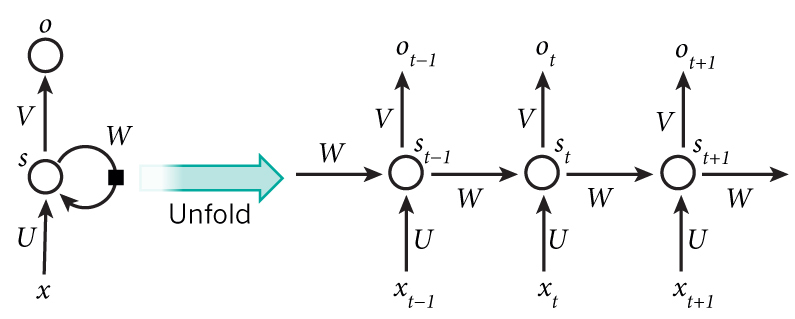
\includegraphics[width=\textwidth]{rnn}
  \caption{RNN schematics}
  \label{fig:rolled_rnn}
\end{figure}

\subsection{Convolutional Neural Networks}

The CNN we will use will be highly specialised for our case. We use the WaveNet
as laid out in the paper by DeepMind.

WaveNet works on data of the form $\bm{x}$, were we describe the distribution as
\begin{equation*}
p(\bm{x}) = \prod_{l=1}^L p(\bm{x}_l| \bm{x}_1, \dots, \bm{x}_{l-1})
\end{equation*}
which is the form common in NLP and NMT. The output of the model has the same
time dimensionality as the input, meaning that the model has the ability to
output a categorical distribution over the next value $x_l$ with a softmax
layer. In our case this is a parametrisation of the output probability at point $l$.

An important part is that it used dilated convolutions, convolution where the filter
is applied to an area larger than its length by skipping input values with a certain
step. Stacking the dilation layers with dilations being powers of 2 leads to output
of the same dimensions as the input. This configuration of dilation factor results
in exponential receptive field growth with depth (CITE WAVENET PAPER).

\section{Natural Language Processing}

Humans use natural language every day to convey concepts and abstractions to each
other in an efficient manner. Compared to formal languages found in
mathematics and programming, the natural languages we use are often
ambiguous systems filled with rules and exceptions\cite{Rosenfeld00twodecades, sep-computational-linguistics}.

Natural Language Processing is an old field that for a long
time developed in parallel with the field of machine learning and
computational statistics which deals with how to process information coming from
human languages and is split up into several subfields such as Machine
Translation, statistical parsing and sentiment analysis\cite{sep-computational-linguistics}.

\subsection{Language model}
We define a sentence to be a vector of words $\bm{w}_{1:L} = (\mathsf{w}_1, \dots,
\mathsf{w}_l)^{\top}$ such that each word is an atomic element $\mathsf{w}_i \in
V$, where $V$ is the dictionary of words in our language. Then the joint
distribution of a word with respect to the underlying probability measure can be
rolled out using the probabilistic chain rule which is just repeated application
of the original product rule in equation \eqref{eq:product_rule}
\begin{equation}
  \label{eq:conditional_language_probability}
  P(\bm{w}_{1:L}) = \prod_{l = 1}^LP(\mathsf{w}_l | \mathsf{w}_1, \dots, \mathsf{w}_{l-1})
\end{equation}
where $\mathsf{w}_l$ is the $l$'th word of the sentence $\bm{w}_{1:L}$\cite{Bengio:2003:NPL:944919.944966}.

\subsection{Word embeddings}
Breaking down sentences at a word level and processing them into a form that
encodes information efficiently is a problem which has gained notorious
recognition, leading to algorithms such as word2vec and
Glove\cite{DBLP:journals/corr/abs-1301-3781, Pennington14glove:global,
  Mikolov:2013:DRW:2999792.2999959}. However, these techniques work less well in
a neural network setting where instead finding the best embedding jointly with
the parameters of the model is peqreferred \cite[p.~5-7]{goldberg2015primer}.

A straightforward way to represent the various words of the dictionary is as
one-hot-encoded vectors such that a word $\mathsf{w} \in V$, such that size of
$V$ is $|V|$, with an index $i$ given by its place in the dictionary sorted
alphabetically in descending order will have the vector representation
\begin{equation}
  \label{eq:one_hot_encoding}
  \bm{w} =
  \begin{bmatrix}
    0 \\
    \vdots \\
    0 \\
    1 \\
    0 \\
    \vdots \\
    0
  \end{bmatrix}
\end{equation}\cite[p.~6]{goldberg2015primer}
such that $\bm{w}_{j} = \delta_{ij}$.

While this is a form conceptually easy to understand, it fails to account for the
curse of dimensionality as the size of the vocabulary might grow to millions of
entries and the fact that the cosine similarity of two words $\mathsf{v}_1,
\mathsf{v}_2 \in V$ is zero unless they are the same word
\begin{equation}
  \label{eq:cosine_similarity}
  \cos_{similarity}(\bm{v}_1, \bm{v}_2) = \delta_{\mathsf{v}_1 \mathsf{v}_2}
\end{equation}. This means that no meaning is embedded in the vector space
except for the location in the sorted dictionary. Instead we would like to
associate each word in the vocabulary with a distributed \textit{word feature
  vector}, a dense, real-valued vector in $\mathbb{R}^m$. Express the joint probability
function \eqref{eq:conditional_language_probability} of word sequences of a
sentence in terms of the feature vectors of these words in the sequence and
simultaneously learn the word feature vectors and the parameters of the model
which dictates the form of the probability function, $\bm{\theta}$. After this
is done words which share similarities in some sense such as \texttt{Dog, Puppy}
would have a higher similarity score than unrelated concepts such as \texttt{Dog, Bulwark}\cite{Bengio:2003:NPL:944919.944966}.

We may represent this in a mathematical form by trying to find a linear map $C$
from any element $\mathsf{w} \in V$ such that $C(\mathbf{w}) \in \mathbb{R}^m$.
Using the usual canonical basis of an Euclidean space, we can express this
linear map in terms of a matrix $\bm{C} \in \mathbb{R}^{m \times |V|}$, thus the
word feature vector of the learned embedding can be represented by the matrix
multiplication $\bm{C}\bm{w}$.

\subsection{Neural machine translation}
For a long time the dominant paradigm within machine translation was to use
phrase based machine translation systems\cite{Koehn:2003:SPT:1073445.1073462,
  Koehn:2007:MOS:1557769.1557821}, however since a couple of year back,
modelling the word or character level directly with neural networks, so called
NMT has become the best performing method\cite{wolk_neural-based_2015, wu_googles_2016}.

Most NMT models work in terms of an encoder-decoder architecture where the
encoder extracts a fixed length representation $\bm{c}$, often called a context
vector, from a variable length input sentence $\bm{x} \in \lang{X}$, and the
decoder uses this representation to generate a correct translation $\bm{y} \in
\lang{Y}$ from this representation\cite{cho_properties_2014}.

\begin{figure}[H]
  \includestandalone[width=\textwidth]{./scripts/tikz_code/encoder_decoder}% 
    \caption{Encoder decoder schematic}
  \label{fig:encoder_decoder}
\end{figure}

\section{Optimization}

\subsection{Problem formulation}

Numerical optimization has been applied to many parts of science and thus many
different algorithms have been developed to tackle different problems. However,
most of the theoretical results that exist deal with convex optimization, where
the function we are trying to optimize is particularly well-behaved, leading to
theoretical guarantees on the solution converged to. The surface of the function
we are trying to optimize in machine learning in general and deep learning in
particular is not well-behaved, being highly non-linear and non-convex, meaning
most theoretical results that exist do not apply to this domain\cite{choromanska_loss_2014}.

Nevertheless, while theoretical results are lacking, there has been substantial
advances in various optimisation techniques fit to attack the highly non-linear,
non-convex and high-dimensional optimization problems of learning in deep
models, particularly from the Stochastic Gradient Descent. This has led to
numerous gradient descent-like algorithms used machine learning\cite{Ruder17}.

\subsection{Stochastic Gradient Descent}

For a normal probabilistic machine learning problem, we have data $\mathcal{D}$
that we try to model with a model $\mathcal{M}$ parametrised by parameters
$\bm{\theta} \in \Theta$. The optimization problem can in the most general case be recast
as an effort to find the parameters $\bm{\theta}_{ML}$ that maximizes the
log-likelihood function \eqref{eq:log-likelihood}.

As this can't be found analytically we have to resort to numerical schemes to
find good candidates which hopefully will be close to the true solution
$\bm{\theta}_{ML}$. The first candidate is called Gradient Descent (GD).
GD approximates the gradient as if it was linear and takes steps to maximize the
probability through a hill-climbing scheme. If we let $\mathcal{D} =
\{\bm{z}_i\}_{i = 1}^n$ such that $\bm{z_i}$ is any general datapoint, $Q$ an
objective function that we try to maximize, such that $Q : \Theta \times
\mathcal{Z} \to \mathbb{R}$, then the update using GD looks as follows
\begin{equation}
  \label{eq:GD_update}
  \bm{\theta}_{t + 1} = \bm{\theta}_t - \gamma_t \frac{1}{n} \sum_{i = 1}^n \nabla_{\bm{\theta}} Q(z_i, \bm{\theta}_t)
\end{equation}.
While $\gamma_t$ may vary with $t$, it is often fixed for practical reasons. As
we can see GD takes into account all of the datapoints in the set, in some sense
updating the parameters with respect to the true linear approximation of the gradient.

However, with the huge size of data existing today, it is often not feasible to
calculate the update for all datapoints in the dataset due to the time it would
take and memory it would take to store the gradients.

Stochastic Gradient Descent is a similar algorithm to GD that instead of
calculating the gradient with respect to the whole dataset calculates an
approximate gradient, hence the word \textit{stochastic}, as it picks a random
subset of the dataset to update $\bm{\theta}$ with regards to. If we let $I_t$
be a random subset of the indices of $V$ of size $m$ then SGD does the
following update
\begin{equation}
  \label{eq:SGD_update}
  \bm{\theta}_{t + 1} = \bm{\theta}_t - \gamma_t \frac{1}{m} \sum_{i \in I_t} \nabla_{\bm{\theta}} Q(z_i, \bm{\theta}_t)
\end{equation}\cite{series/lncs/Bottou12}\cite[p.~240]{Bishop:2006}.

The stochasticity has been shown to act as a regularizer and several analyses of
this in terms of a Bayesian framework has been done, explaining the stationary
behaviour of SGD with constant learning rate after convergence
\cite{mandt_stochastic_2017, mandt_variational_2016}.

\subsection{ADAM}
SGD has found widespread use within the machine learning community due to strong
experimental results and ease of use, especially in deep learning. Lately
though, a number of alternatives have sprung up that aims to improve the vanilla
SGD, such as RMSProp\cite{Tieleman2012} and AdaGrad\cite{Duchi:EECS-2010-24}.

Adam takes inspiration from RMSProp and AdaGrad. Technically, Adam keeps an
exponential running average of the first and second order statistics of the
gradient, using these to calculate an adaptive learning rate.

As laid out in the original paper, ADAM operates on a stochastic objective
function $f(\bm{\theta})$, which in our case would be the probability averaged
over our input batch. $f_t(\bm{\theta})$ denotes this function over different
timesteps, equally $g_t = \nabla_{\bm{\theta}} f_t(\bm{\theta})$. $m_t$ and
$v_t$ denotes the first and second order moments of the gradients, however,
these are biased and are corrected in the algorithm.

The whole algorithm is as follows.

\begin{algorithm}
  \caption{ADAM}\label{ADAM}
  \begin{algorithmic}[1]
    \Require $\alpha$: Stepsize
    \Require $\beta_1, \beta_2 \in [0, 1)$: Exponential decay rates of the moment estimates
    \Require $f(\bm{\theta})$: Stochastic objective function with parameters
    $\bm{\theta}$
    \Require $\bm{\theta}_0$: Initial parameter vector
    \State $m_0 \gets 0$ (Initialize $1^{\text{st}}$ moment vector)
    \State $v_0 \gets 0$ (Initialize $2^{\text{nd}}$ moment vector)
    \State $t \gets 0$ (Initialize timestep)
    \While{$\bm{\theta}_t$ not converged}
    \State $t \gets t + 1$
    \State $g_t \gets \nabla_{\bm{\theta}}f_t(\bm{\theta}_{t-1})$ (get gradients w.r.t stochastic objective at timestep $t$)
    \State $m_t \gets \beta_1 \cdot m_{t-1} + (1 - \beta_1) \cdot g_t$ (Update biased first moment estimate)
    \State $v_t \gets \beta_2 \cdot v_{t-1} + (1 - \beta_2) \cdot g^2_t$ (Update biased second raw moment estimate)
    \State $\hat{m}_1 \gets m_t / (1 - \beta^t_1)$ (Compute bias-corrected first moment estimate)
    \State $\hat{v}_1 \gets v_t / (1 - \beta^t_2)$ (Compute bias-corrected second raw moment estimate)
    \State $\bm{\theta}_t \gets \bm{\theta}_{t-1} - \alpha \cdot \hat{m}_i/(\sqrt{\hat{v}_t} + \epsilon)$ (Update parameters)
    \EndWhile
    \Return $\bm{\theta}_t$ (Resulting parameters)
  \end{algorithmic}
\end{algorithm}

Experimentally Adam has shown very good results on training various deep
learning models such as MLP's, CNN's and RNN's so we will use it to train our
models throughout this dissertation\cite{kingma_adam:_2014}.